Les objectifs du premier hands-on sont:
\begin{itemize}
	\item[-] De se familiariser avec le matérial de base (breadboard, multimètre, oscilloscope) et les composants de base (résistances, capacités, amplificateurs opérationnels, composants intégrés) propres à l'électronique.
	\item[-] D'implémenter et de comprendre le fonctionnement du contrôle du volume audio, sur base du signal délivré par l'ordinateur ou le smartphone.
	\item[-] D'interfacer ce circuit avec un buzzer piézoélectrique ou un baffle pour entendre le son ainsi produit.
\end{itemize}

\begin{figure}[!ht]
	\centering
	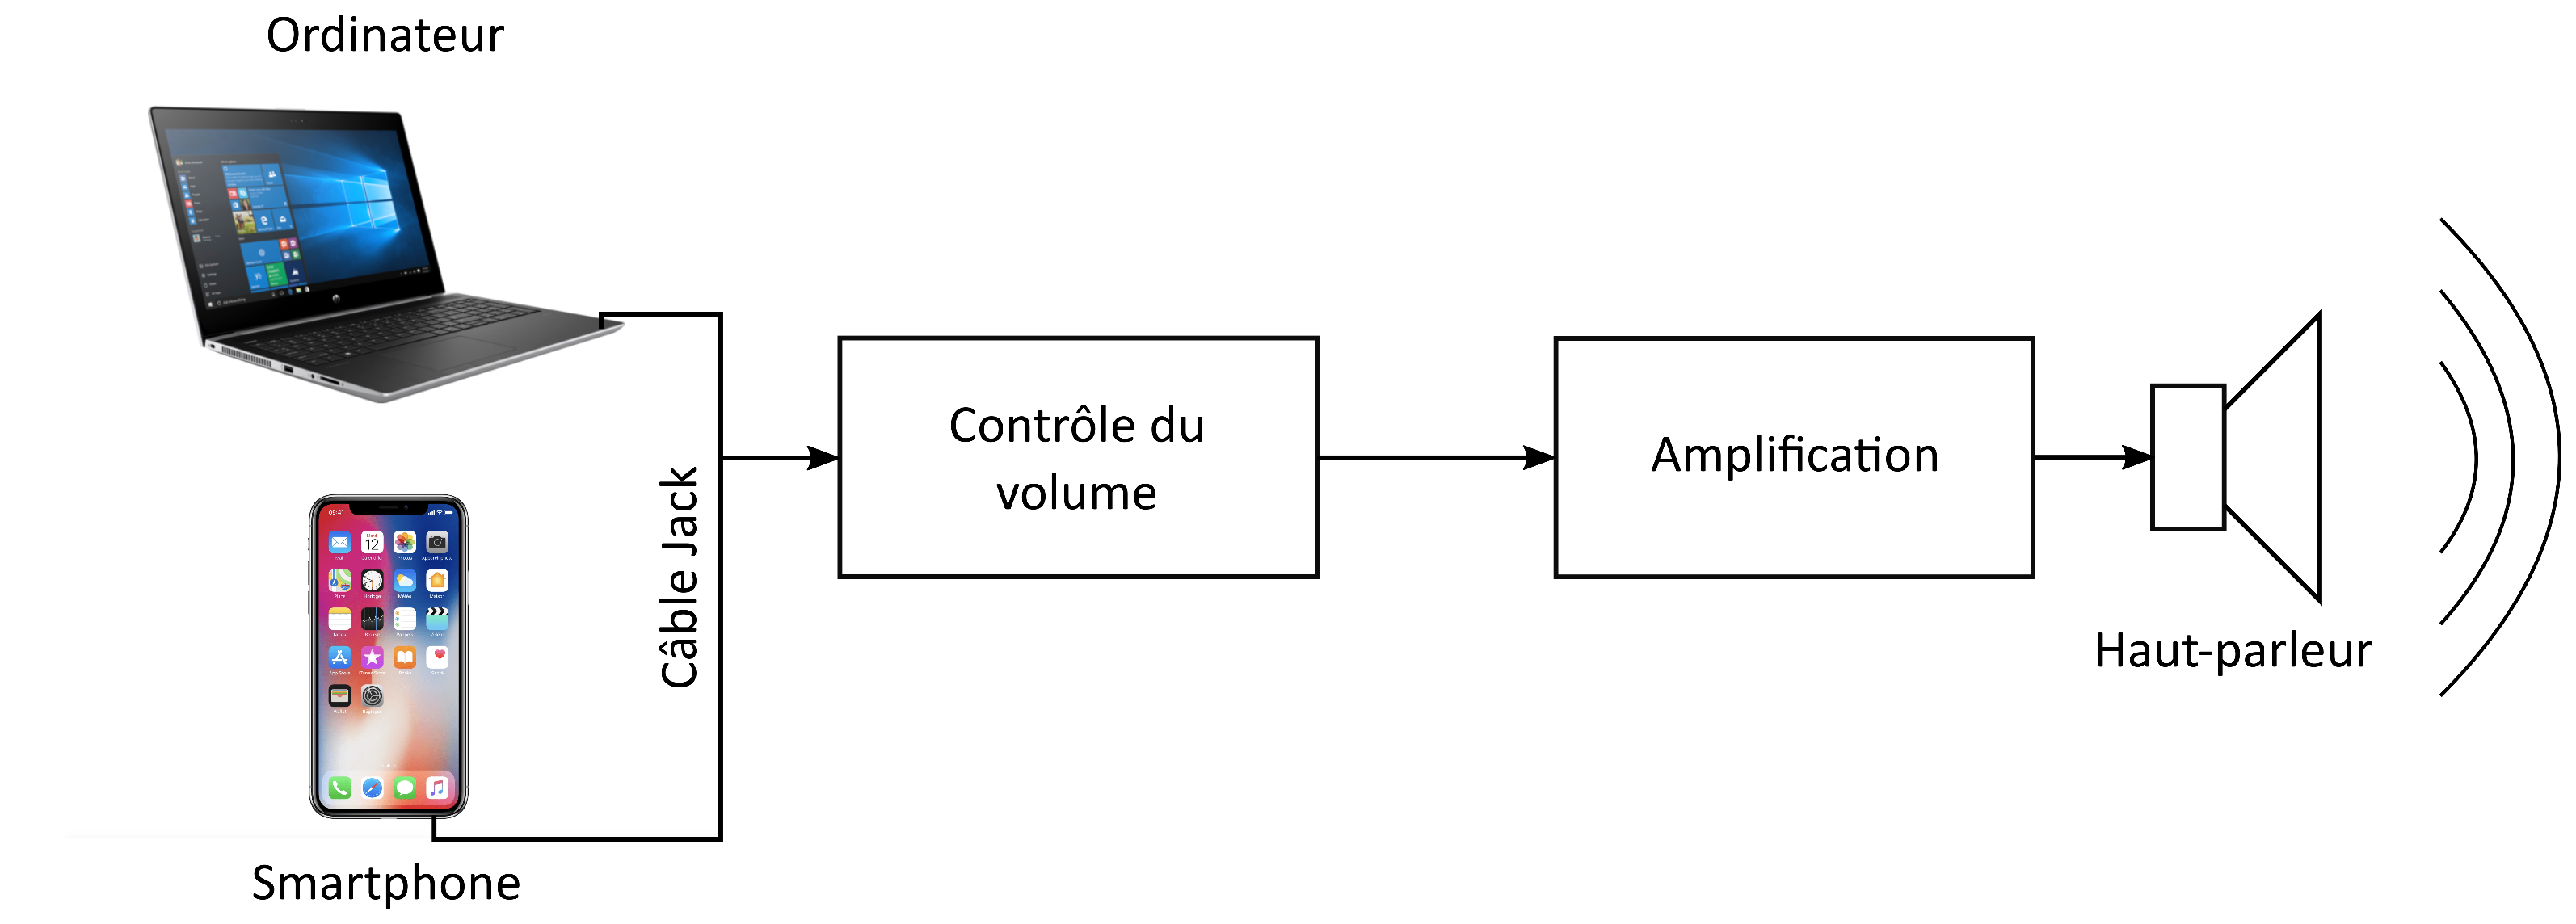
\includegraphics[width=.75\textwidth]{figures/block-diagram.eps}
	\caption{Schéma-bloc du circuit.}
	\label{fig:block-diagram}
\end{figure}

Le schéma-bloc du circuit est présenté à la Figure \ref{fig:block-diagram}. Le signal audio produit par l'ordinateur ou smartphone est branché au circuit au travers d'un câble Jack. L'amplitude de ce signal est ensuite modifiée dans le bloc de contrôle du volume grâce à une diviseur résistif, qui sera détaillé plus loin dans ce document. Un bloc d'amplification, consistant en amplificateur de puissance, est finalement nécessaire pour pouvoir se connecter à un baffle.